\documentclass[12pt]{article}
\usepackage{amsfonts, amssymb, amsmath, amsthm}
\usepackage[margin=1in]{geometry}
\usepackage{tikz}
\usetikzlibrary{patterns, decorations.pathreplacing, arrows.meta}

\pagestyle{myheadings}
\markright{Explainer: Rudin 2.29 — Open Sets in $\mathbb{R}$\hfill}

\newcommand{\R}{\mathbb{R}}
\newcommand{\Q}{\mathbb{Q}}
\newcommand{\N}{\mathbb{N}}

\begin{document}

\begin{center}
    \textbf{\Large Open Sets in $\mathbb{R}$ are Countable Unions of Disjoint Segments}\\[0.5em]
    \large A visual guide to Rudin 2.29
\end{center}

\section{The Claim}

Every open set $G \subseteq \mathbb{R}$ can be written as:
\[
G = \bigcup_{n=1}^{\infty} I_n
\]
where the $I_n$ are \textbf{disjoint open intervals} (segments), and there are \textbf{at most countably many} of them.

\section{What Do Open Sets in $\mathbb{R}$ Look Like?}

\begin{center}
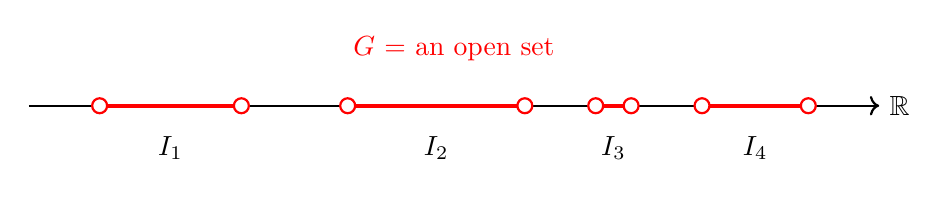
\begin{tikzpicture}[scale=0.9]
    \draw[thick, ->] (-6, 0) -- (6, 0) node[right] {$\mathbb{R}$};

    % An open set G with gaps
    \draw[red, ultra thick] (-5, 0) -- (-3, 0);
    \draw[red, ultra thick] (-1.5, 0) -- (1, 0);
    \draw[red, ultra thick] (2, 0) -- (2.5, 0);
    \draw[red, ultra thick] (3.5, 0) -- (5, 0);

    % Open endpoints
    \draw[red, thick, fill=white] (-5, 0) circle (3pt);
    \draw[red, thick, fill=white] (-3, 0) circle (3pt);
    \draw[red, thick, fill=white] (-1.5, 0) circle (3pt);
    \draw[red, thick, fill=white] (1, 0) circle (3pt);
    \draw[red, thick, fill=white] (2, 0) circle (3pt);
    \draw[red, thick, fill=white] (2.5, 0) circle (3pt);
    \draw[red, thick, fill=white] (3.5, 0) circle (3pt);
    \draw[red, thick, fill=white] (5, 0) circle (3pt);

    \node[red] at (0, 0.8) {$G$ = an open set};

    % Labels for intervals
    \node at (-4, -0.6) {$I_1$};
    \node at (-0.25, -0.6) {$I_2$};
    \node at (2.25, -0.6) {$I_3$};
    \node at (4.25, -0.6) {$I_4$};
\end{tikzpicture}
\end{center}

Open sets in $\mathbb{R}$ can have ``gaps'' — points not in the set. The set naturally breaks into disjoint intervals.

\section{The Key Idea: Maximal Intervals}

For any point $x \in G$, define the \textbf{maximal interval} containing $x$:
\[
I_x = \text{the largest open interval containing } x \text{ that is still contained in } G
\]

\begin{center}
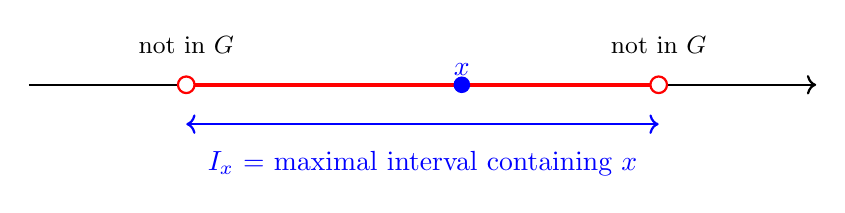
\begin{tikzpicture}[scale=1]
    \draw[thick, ->] (-5, 0) -- (5, 0);

    % The open set G
    \draw[red, ultra thick] (-3, 0) -- (3, 0);
    \draw[red, thick, fill=white] (-3, 0) circle (3pt);
    \draw[red, thick, fill=white] (3, 0) circle (3pt);

    % Point x
    \fill[blue] (0.5, 0) circle (3pt) node[above] {$x$};

    % Show the maximal interval
    \draw[blue, thick, <->] (-3, -0.5) -- (3, -0.5);
    \node[blue] at (0, -1) {$I_x$ = maximal interval containing $x$};

    % Endpoints are NOT in G
    \node at (-3, 0.5) {\small not in $G$};
    \node at (3, 0.5) {\small not in $G$};
\end{tikzpicture}
\end{center}

\textbf{How to construct $I_x$:}
\begin{align*}
a_x &= \inf\{a : (a, x) \subseteq G\} \\
b_x &= \sup\{b : (x, b) \subseteq G\}
\end{align*}
Then $I_x = (a_x, b_x)$.

\section{Key Properties of Maximal Intervals}

\subsection{Property 1: They Cover $G$}

Every point $x \in G$ is in its maximal interval $I_x$, so:
\[
G = \bigcup_{x \in G} I_x
\]

\subsection{Property 2: They're Either Equal or Disjoint}

\begin{center}
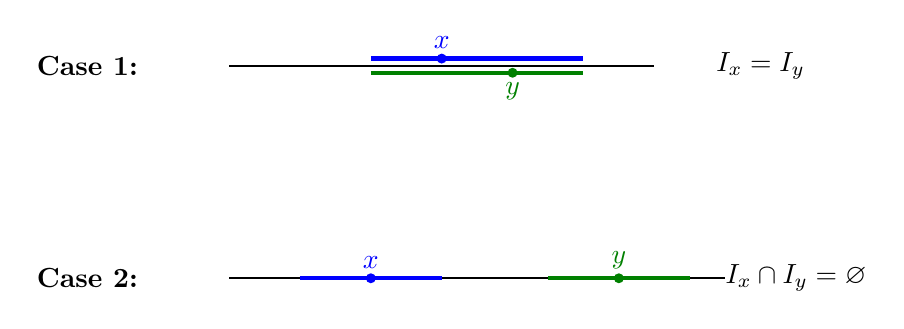
\begin{tikzpicture}[scale=0.9]
    % Case 1: Equal
    \begin{scope}[yshift=1.5cm]
        \node at (-4, 0) {\textbf{Case 1:}};
        \draw[thick] (-2, 0) -- (4, 0);
        \draw[blue, ultra thick] (0, 0.1) -- (3, 0.1);
        \draw[green!50!black, ultra thick] (0, -0.1) -- (3, -0.1);
        \fill[blue] (1, 0.1) circle (2pt) node[above] {$x$};
        \fill[green!50!black] (2, -0.1) circle (2pt) node[below] {$y$};
        \node at (5.5, 0) {$I_x = I_y$};
    \end{scope}

    % Case 2: Disjoint
    \begin{scope}[yshift=-1.5cm]
        \node at (-4, 0) {\textbf{Case 2:}};
        \draw[thick] (-2, 0) -- (5, 0);
        \draw[blue, ultra thick] (-1, 0) -- (1, 0);
        \draw[green!50!black, ultra thick] (2.5, 0) -- (4.5, 0);
        \fill[blue] (0, 0) circle (2pt) node[above] {$x$};
        \fill[green!50!black] (3.5, 0) circle (2pt) node[above] {$y$};
        \node at (6, 0) {$I_x \cap I_y = \varnothing$};
    \end{scope}
\end{tikzpicture}
\end{center}

\textbf{Why?} If $I_x$ and $I_y$ overlap but aren't equal, their union $I_x \cup I_y$ would be a larger interval contained in $G$ — contradicting maximality!

\begin{center}
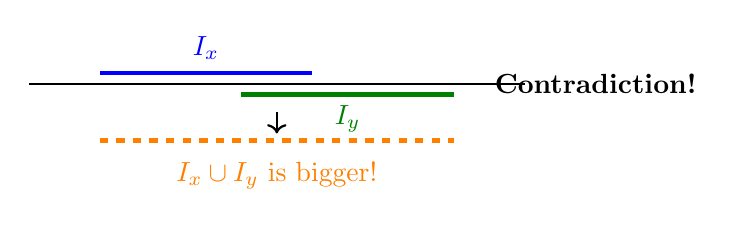
\begin{tikzpicture}[scale=0.9]
    \draw[thick] (-1, 0) -- (6, 0);

    % Overlapping intervals
    \draw[blue, ultra thick] (0, 0.15) -- (3, 0.15);
    \draw[green!50!black, ultra thick] (2, -0.15) -- (5, -0.15);

    \node[blue] at (1.5, 0.5) {$I_x$};
    \node[green!50!black] at (3.5, -0.5) {$I_y$};

    % Their union
    \draw[orange, ultra thick, dashed] (0, -0.8) -- (5, -0.8);
    \node[orange] at (2.5, -1.3) {$I_x \cup I_y$ is bigger!};

    \draw[->, thick] (2.5, -0.4) -- (2.5, -0.7);
    \node at (7, 0) {\textbf{Contradiction!}};
\end{tikzpicture}
\end{center}

\section{So We Have Disjoint Intervals — Why Countably Many?}

This is where the hint comes in: use the fact that $\mathbb{R}$ is \textbf{separable} (from Problem 2.22).

\begin{center}
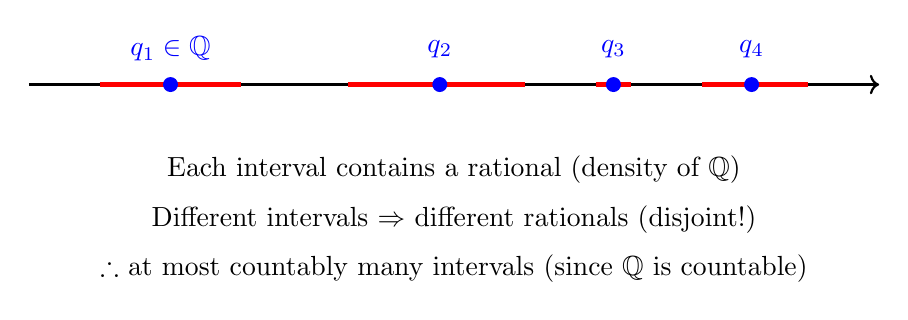
\begin{tikzpicture}[scale=0.9]
    \draw[thick, ->] (-6, 0) -- (6, 0);

    % Disjoint intervals
    \draw[red, ultra thick] (-5, 0) -- (-3, 0);
    \draw[red, ultra thick] (-1.5, 0) -- (1, 0);
    \draw[red, ultra thick] (2, 0) -- (2.5, 0);
    \draw[red, ultra thick] (3.5, 0) -- (5, 0);

    % Rational in each
    \fill[blue] (-4, 0) circle (3pt);
    \fill[blue] (-0.2, 0) circle (3pt);
    \fill[blue] (2.25, 0) circle (3pt);
    \fill[blue] (4.2, 0) circle (3pt);

    \node[blue] at (-4, 0.5) {$q_1 \in \mathbb{Q}$};
    \node[blue] at (-0.2, 0.5) {$q_2$};
    \node[blue] at (2.25, 0.5) {$q_3$};
    \node[blue] at (4.2, 0.5) {$q_4$};

    \node at (0, -1.2) {Each interval contains a rational (density of $\mathbb{Q}$)};
    \node at (0, -1.9) {Different intervals $\Rightarrow$ different rationals (disjoint!)};
    \node at (0, -2.6) {$\therefore$ at most countably many intervals (since $\mathbb{Q}$ is countable)};
\end{tikzpicture}
\end{center}

\textbf{The Argument:}
\begin{enumerate}
    \item Each maximal interval $I$ is nonempty and open, so it contains a rational $q_I \in \mathbb{Q}$ (by density).
    \item If $I \neq J$ are two distinct maximal intervals, they're disjoint, so $q_I \neq q_J$.
    \item This gives an injection from $\{\text{maximal intervals}\}$ to $\mathbb{Q}$.
    \item Since $\mathbb{Q}$ is countable, there are at most countably many maximal intervals.
\end{enumerate}

\section{Summary of the Proof}

\begin{enumerate}
    \item For each $x \in G$, define $I_x = (a_x, b_x)$ where:
    \begin{align*}
        a_x &= \inf\{a : (a, x) \subseteq G\} \\
        b_x &= \sup\{b : (x, b) \subseteq G\}
    \end{align*}

    \item Show $I_x \subseteq G$ (need to verify this!)

    \item Show: if $I_x \cap I_y \neq \varnothing$, then $I_x = I_y$

    \item Conclude: the distinct maximal intervals partition $G$

    \item Each interval contains a rational; different intervals contain different rationals

    \item Therefore: at most countably many intervals
\end{enumerate}

\section{A Subtlety: Why is $I_x \subseteq G$?}

We need to check that $(a_x, b_x) \subseteq G$.

Let $y \in (a_x, b_x)$. Then $a_x < y < b_x$.

\begin{itemize}
    \item Since $y > a_x = \inf\{a : (a, x) \subseteq G\}$, there exists $a < y$ with $(a, x) \subseteq G$.
    \item Since $y < b_x = \sup\{b : (x, b) \subseteq G\}$, there exists $b > y$ with $(x, b) \subseteq G$.
    \item So $(a, x) \cup (x, b) = (a, b) \setminus \{x\} \subseteq G$, and $x \in G$.
    \item Therefore $(a, b) \subseteq G$, and since $a < y < b$, we have $y \in G$.
\end{itemize}

\section{Visual Summary}

\begin{center}
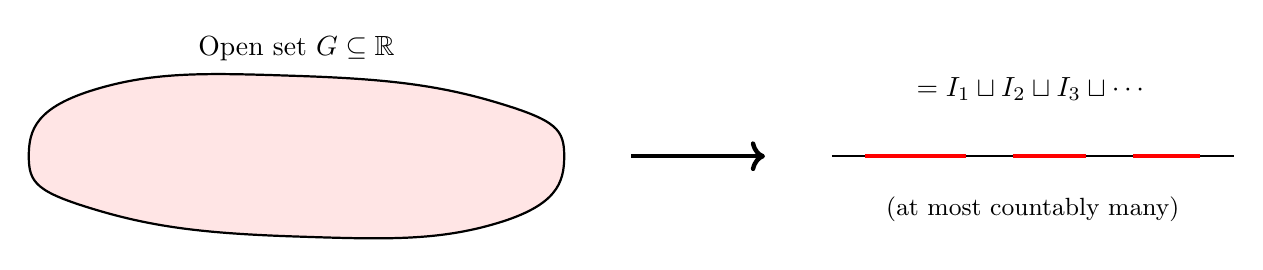
\begin{tikzpicture}[scale=0.85]
    % Open set G
    \draw[thick, fill=red!10] plot[smooth cycle, tension=0.8] coordinates {(-4,0) (-3,1) (0,1.2) (3,0.8) (4,0) (3,-1) (0,-1.2) (-3,-0.8)};
    \node at (0, 1.6) {Open set $G \subseteq \mathbb{R}$};

    \draw[->, ultra thick] (5, 0) -- (7, 0);

    % Decomposition
    \begin{scope}[xshift=11cm]
        \draw[thick] (-3, 0) -- (3, 0);
        \draw[red, ultra thick] (-2.5, 0) -- (-1, 0);
        \draw[red, ultra thick] (-0.3, 0) -- (0.8, 0);
        \draw[red, ultra thick] (1.5, 0) -- (2.5, 0);

        \node at (0, 1) {$= I_1 \sqcup I_2 \sqcup I_3 \sqcup \cdots$};
        \node at (0, -0.8) {\small (at most countably many)};
    \end{scope}
\end{tikzpicture}
\end{center}

\end{document}
